\section{Introduction}
\label{sec:intro}

\begin{figure}[t]
  \centering
  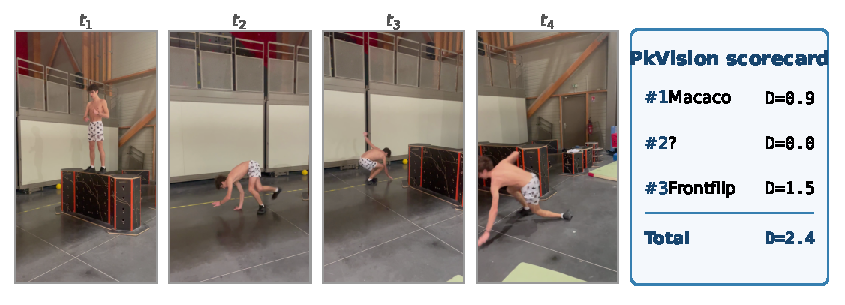
\includegraphics[width=\linewidth]{figures/fig01_teaser.pdf}
  \caption{\textbf{\sys{} at a glance.} Four frames from a real
  competition run (\texttt{IMG\_5985.mov}) are segmented into individual
  tricks by an inversion signal, passed through a vision--language
  model, fuzzy-matched to the FIG Parkour Code of Points 2025 table,
  and assembled into a D-score card. The scorecard here shows the
  ground-truth tricks for the run; Sec.~\ref{sec:experiments} reports
  what the VLMs actually returned on the matching segments.}
  \label{fig:teaser}
\end{figure}

Parkour has grown from a street practice into a FIG
World-Championship discipline in under a decade, and is under
discussion for inclusion in future Olympic programmes. Its scoring
system, the 2025--2028 Code of Points~\cite{fig2025codepoints},
defines 149 named tricks across four categories (swing, wall,
acrobatics, parkour basics) and assigns each a base difficulty value.
A run's D-score is the sum of the three highest matched base values;
its E-score covers execution and deductions. Even experienced human
judges disagree on trick identity when rotations exceed two
revolutions or when multiple twists are chained together, and the
pool of qualified FIG judges is a structural bottleneck for scaling
the discipline~\cite{fig2025codepoints,
internationalparkour2024judges}.

Automated judging exists for adjacent
disciplines---Fujitsu's gymnastics Judging Support
System~\cite{fujitsu2023jss} and several ISU pilots for figure
skating~\cite{isu2023automation}---but all depend on bespoke
multi-camera rigs, closed datasets, and per-element engineering.
No open-source equivalent exists for parkour, and the 149-entry FIG
table itself is only three years old. The practical question we
address is: \emph{what does an end-to-end, monocular, zero-shot FIG
D-scoring system look like today, and how well does it actually work?}

We report three things in this paper, all honest.

\paragraph{A system.}
\sys{} is a modular pipeline: YOLO-pose tracking, inversion-based
trick segmentation (Sec.~\ref{sec:system:segmentation}), an
off-the-shelf vision--language model with a FIG-grounded prompt
(Sec.~\ref{sec:system:vlm}), a five-level fuzzy matcher that snaps
free-form VLM output onto the 149 FIG entries
(Sec.~\ref{sec:system:matcher}), and a deterministic D-score
assembler. Every stage has a text-level interface and is auditable.
The components do not share a learned representation, and each can be
replaced without retraining anything. The system is released
open-source at \url{https://github.com/AirKyzzZ/pkvision}.

\paragraph{A journey.}
Before arriving at the VLM pipeline we spent eighteen months on five
trained-model approaches that did not work: 2D pose plus hand-crafted
physics (brittle under camera motion), a 3D human mesh recovery
pipeline built on GVHMR~\cite{shen2024gvhmr} (its AMASS~\cite{mahmood2019amass}
training data contains zero acrobatic sequences, producing garbage
rotations on competition footage), metric learning on 1\,618 labeled
parkourtheory.com clips (R@1 of 9\% with embedding collapse),
hierarchical attribute classifiers on a VideoMAE~\cite{tong2022videomae}
backbone (55\% mean accuracy at six epochs before a cluster timeout),
and CLIP~\cite{radford2021clip} zero-shot (37--48\% on coarse
attributes, 0\% on exact trick names). Section~\ref{sec:journey}
documents each failure, because every one of them points to a design
decision in the system we ended up with.

\paragraph{An honest evaluation.}
We evaluate \sys{} on 13 curated single-trick clips (POOL-B) with
ground-truth FIG labels assigned by the author using a lightweight
web interface we release with the paper. We benchmark three VLM
configurations: Claude Sonnet~4.5 via a composite 8-frame strip
through the Claude Code CLI, Gemini~2.5 Flash via native video
ingestion through the Google Generative AI SDK, and Qwen2.5-VL~72B
via OpenRouter. None of them achieve strong top-1 accuracy in our
headless automation pipeline---their best result is roughly one in
five single-trick clips identified correctly---even though the same
models routinely succeed on the same clips when a human queries them
interactively through a chat interface. We document this
\emph{automation gap}, catalogue the recurring failure modes
(twist under-counting, takeoff confusion, wall-context loss), and
show that the fuzzy matcher and the inversion segmenter remain
useful regardless of which VLM is plugged in.

\paragraph{Contributions.}
\begin{itemize}
  \setlength\itemsep{-2pt}
  \item \textbf{\sys{}}, an open-source, monocular, zero-shot FIG
        D-scoring pipeline, released with all code, prompts, FIG
        table, and ground-truth labels.
  \item An \textbf{inversion-based trick segmenter} that splits real
        competition runs into per-trick clips using only 2D keypoint
        signals, and therefore does not inherit the acrobatic blind
        spot of current 3D human-mesh recovery models. It cleanly
        isolates the three tricks of our reference run
        \texttt{IMG\_5985.mov} from its run-ups and transitions
        (Fig.~\ref{fig:segmentation}).
  \item A \textbf{five-level fuzzy FIG matcher} that maps free-form
        VLM output to the 149-entry FIG Table of Tricks, auditable
        at every hop.
  \item An \textbf{empirical study} showing that frontier VLMs in
        headless automation mode currently achieve low top-1 accuracy
        on FIG parkour tricks, with qualitative consistency across
        models (Gemini~2.5 Flash, Claude Sonnet~4.5, Qwen2.5-VL~72B),
        and a catalogue of the recurring failure modes.
  \item A \textbf{pragmatic journey} through five trained-model
        approaches that did not work, kept short on purpose and
        mapped to the design decisions they motivated.
\end{itemize}

We explicitly make no claim that \sys{} replaces a human judge. Our
goal is to produce a system that is \emph{good enough to be built on}
by the parkour community, honest enough to be audited, and modular
enough to let a future VLM or a future physics module drop in without
rewriting the pipeline.
